{
    \subsection{Հարցումների համակարգ}\label{subsec:queries}

    Երկրորդ փուլում նախագծվել է բուն հարցումների համակարգը:
    Նախագծված համակարգը հանդիսանում է ծրագրային կոդի հատկությունների վերլուծության կարևոր բաղկացուցիչ մասը:
    Հարցումների համակարգը ճկուն է, ընդլայնելի և հեշտ օգտագործվող:
    Այս համակարգը թույլ է տալիս ծրագրավորողներին, նույնիսկ առանց խորը վերլուծական գիտելիքների,
    արագ և ճշգրիտ ստանալ տեղեկատվություն իրենց ծրագրերի կառուցվածքի և հատկությունների մասին:

    Նախագծված API-ի միջոցով օգտագործողները կարող են կատարել հարցումներ, որի արդյունքում համակարգը տվյալների բազայից վերցնում է անհրաժեշտ
    տվյալներ, կատարում համապատասխան վերլուծություններ և տալիս է հարցմումների պատասխանները (Նկար \ref{fig:figure6}):

    \begin{figure}[h]
        \centering
        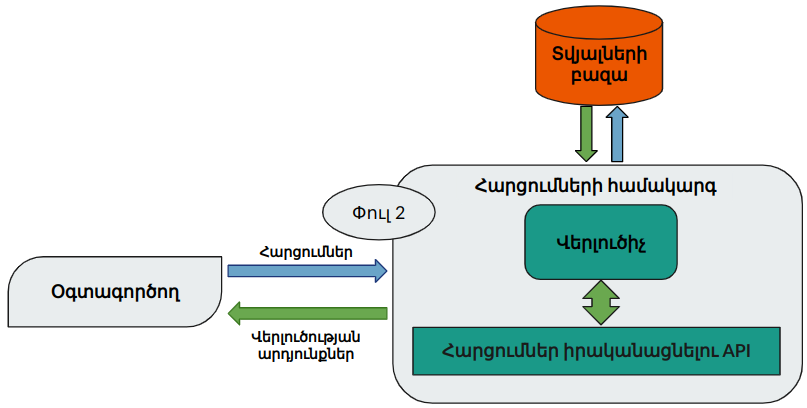
\includegraphics[width=1\textwidth]{pic6}
        \caption{Փուլ 2, Հարցումների համակարգ}
        \label{fig:figure6}
    \end{figure}

    {
    \subsubsection{Հարցումների խմբեր}\label{subsubsec:queryGroups}
    Գրել բաժանումների մասին

    \phantomsection
    \subsubsection*{Դասերի համար հարցումներ}\label{subsubsec:classes}
    \addcontentsline{toc}{subsubsection}{Դասերի համար հարցումներ}
    Կլասների հարցումների մասին խոսել։

    \phantomsection
    \subsubsection*{Ֆունկցիաների համար հարցումներ}\label{subsubsec:functions}
    \addcontentsline{toc}{subsubsection}{Ֆունկցիաների համար հարցումներ}
    Ֆունկցիաների հարցումների մասին խոսել։

    \phantomsection
    \subsubsection*{Հրահանգների համար հարցումներ}\label{subsubsec:instructions}
    \addcontentsline{toc}{subsubsection}{Հրահանգների համար հարցումներ}
    Ինստրուկցիաների հարցումների մասին խոսել։

    \phantomsection
    \subsubsection*{Օգտագործողի կողմից կառավարվող տվյալների վերլուծության հարցումներ}\label{subsubsec:taintAnalisys}
    \addcontentsline{toc}{subsubsection}{Օգտագործողի կողմից կառավարվող տվյալների վերլուծության հարցումներ}
    Ավելացնել ալգորիթմերի բարդությունը։
}
}